% -*- latex -*-
%-----------------------------------------------------------------------
%;  Copyright (C) 2002
%;  Associated Universities, Inc. Washington DC, USA.
%;
%;  This program is free software; you can redistribute it and/or
%;  modify it under the terms of the GNU General Public License as
%;  published by the Free Software Foundation; either version 2 of
%;  the License, or (at your option) any later version.
%;
%;  This program is distributed in the hope that it will be useful,
%;  but WITHOUT ANY WARRANTY; without even the implied warranty of
%;  MERCHANTABILITY or FITNESS FOR A PARTICULAR PURPOSE.  See the
%;  GNU General Public License for more details.
%;
%;  You should have received a copy of the GNU General Public
%;  License along with this program; if not, write to the Free
%;  Software Foundation, Inc., 675 Massachusetts Ave, Cambridge,
%;  MA 02139, USA.
%;
%;  Correspondence concerning AIPS should be addressed as follows:
%;          Internet email: aipsmail@nrao.edu.
%;          Postal address: AIPS Project Office
%;                          National Radio Astronomy Observatory
%;                          520 Edgemont Road
%;                          Charlottesville, VA 22903-2475 USA
%-----------------------------------------------------------------------
%Body of intermediate AIPSletter for 31 December 2001

\documentclass[twoside]{article}
\usepackage{graphics}

\newcommand{\AIPRELEASE}{December 31, 2001}
\newcommand{\AIPVOLUME}{Volume XXI}
\newcommand{\AIPNUMBER}{Number 2}
\newcommand{\RELEASENAME}{{\tt 31DEC01}}
\newcommand{\OLDNAME}{{\tt 31DEC00}}
\newcommand{\NEXTNAME}{{\tt 31DEC02}}

%macros and title page format for the \AIPS\ letter.
\input LET98.MAC
%\input psfig

\newcommand{\MYSpace}{-11pt}

\normalstyle

\section{General developments in \AIPS}

\vfill
\subsection{Move of the \AIPS\ home}

Since what remains of the \AIPS\ programming group is now all in
Socorro, we have decided to move all software functions to the Array
Operations center.  The primary address for reaching the \AIPS\ group
remains {\tt daip@nrao.edu}.  The web address will change to {\tt
http://www.aoc.nrao.edu/aips} and the ftp address will become {\tt
ftp://ftp.aoc.nrao.edu/computing/aips}.  Ernie Allen in
Charlottesville will continue to assist the group by handling
registrations, usage statistics, and requests for tapes, CDroms, and
paper documents.  Ernie may be reached at {\tt aipsmail@nrao.edu} for
which he performs triage and at {\tt eallen@nrao.edu}.

The ``Midnight Job'' has been changed.  The secure shell, with all its
fragile complexities, will no longer be required.  Instead {\tt
mnj.aoc.nrao.edu} will serve up \AIPS\ incrementally --- or as a whole
--- using the Unix tool {\tt cvs} running with anonymous ftp.  Linux
sites will almost certainly have {\tt cvs} installed; other sites may
have installed it along with other GNU tools.  Secondary MNJs will
still be possible using {\tt ssh} or {\tt rcp} or NFS as at present.
Further changes to the MNJ will be discussed later in the \Aipsletter.

\vfill
\subsection{Linux news}

RedHat has released versions 7.0, 7.1, and 7.2 of their Linux system.
The good news is that version 7.1 and beyond contain numerous system
improvements including the 2.4.2 kernel.  This kernel allows \AIPS\ to
read and write files larger than 2 Gbytes.  The bad news is that these
releases include and depend on the ``GNU compilers version 2.96.''
The quote marks are added because the GNU compiler group never
released a version 2.96 and they do not support this ``version.''  We
have found that this {\tt g77} produces optimized code that is
unreliable.  There are problems with {\tt IMAGR}, TV window setting,
{\tt TVFLG}, and who knows what else.  We do recommend RedHat release
7.2, but you must also install the GNU compiler suite version 2.95
(now 2.95.3) or 3.0+ (now 3.0.3) --- both of which work well --- and
change your local copies of {\tt FDEFAULT.SH}, {\tt CCOPTS.SH}, and
{\tt FDOPTS.SH} to point at it.  Some other Linux distributions also
include the 2.96 compiler with the same unfortunate results.
Instructions for fetching and installing the real GNU compilers are
given on the \AIPS\ web page.

\vfill\eject
\subsection{Current and future releases}

We have reinstated the old practice of having formal \AIPS\ releases,
but on an annual basis with binary releases only for Solaris and
Linux.  All architectures can do a full installation from the source
files.  The current release is called {\tt 31DEC01} and is now
frozen.  You may fetch a copy of this version from either our
Charlottesville ({\tt www.cv.nrao.edu/aips}) or Socorro ({\tt
www.aoc.nrao.edu/aips}) web sites.  Copies of {\tt 31DEC01} on CDrom or
magnetic tape may be ordered from Ernie Allen at {\tt
aipsmail@nrao.edu}.  This issue of the \Aipsletter\ is intended to
advise you of developments in the last six months in this new release;
the June 30 issue of the \Aipsletter\ covered the first six months.

A new version of \AIPS, called {\tt 31DEC02}, is now under
development by the \AIPS\ Group.  You may fetch (from the aoc web site
only) and install a complete copy of this version at any time.  Having
fetched {\tt 31DEC02}, you may update your installation whenever you
want either as a whole or by running the so-called ``midnight job''
which uses transaction files to copy and compile the code selectively
based on the code changes and compilations we have done.  We expect
users to take the source-only version of \AIPS\ over the Internet (via
\emph{anonymous} ftp).

\AIPS\ is now copyright \copyright\ 1995 through 2002 by Associated
Universities, Inc., NRAO's parent corporation, but may be made freely
available under the terms of the Free Software Foundation's General
Public License (GPL)\@.  This means that User Agreements are no longer
required, that \AIPS\ may be obtained via anonymous ftp without
contacting NRAO, and that the software may be redistributed (and/or
modified), under certain conditions.  The full text of the GPL can be
found in the \texttt{15JUL95} \Aipsletter\ and in the file called {\tt
COPYING} distributed with each release of \AIPS\@.

\section{Improvements of interest to users in \RELEASENAME}

We expect to continue publishing the \Aipsletter\ approximately every
six months with the December \Aipsletter s tied to the annual
releases.  The June 30, 2001 \Aipsletter\ described  a surprising
number of changes in {\tt 31DEC01} over its first six months.  That
\Aipsletter\ described five new tasks: {\tt CHKFC} to check the
contents of an {\tt IMAGR} {\tt BOXFILE}, {\tt DEFLG} to flag data
based on the level of decorrelation, {\tt SNFLG} to flag data on a
baseline basis based on phase jumps in the {\tt SN} or {\tt CL} table,
{\tt VPFLG} to make sure that all polarizations are flagged in a
sample if any are, and {\tt DRCHK} to test the installation control
files for correctness.  A new verb was written called {\tt EPOCONV} to
convert epochs in the {\tt COORDINA} adverb.  New VLBA Utility
procedures also became available.  Significant improvements in {\tt
IMAGR}, {\tt SETFC}, {\tt FILLM}, {\tt FITLD}, {\tt BPASS}, {\tt
PCAL}, {\tt CLCOR}, {\tt SAD}, {\tt TVFLG}, {\tt ZAP}, and others were
described.  That \Aipsletter\ is available from either of the two web
sites above.

In the last six months, the level of activity has been less
surprising.  There is a new procedure {\tt  FITDISK} to write data
using {\tt FITTP} to disk files with names based on the internal file
names.  A new pseudoverb {\tt USAVE} allows the POPS environment to be
saved to another user number.  The new task {\tt RMSD} computes the
local rms in a moving 2-dimensional window.  Wendy Lane and Joe Lazio
of NRL contributed a new task {\tt UVWAX} to delete data based on the
$(u,v,w)$ location.  Bryan Butler has contributed some significant
improvements to {\tt FILLM}\@.  {\tt TECOR} was made more convenient
to use and was discovered to be very helpful even at relatively high
frequencies.

Other than relatively minor differences, {\tt 31DEC01} is compatible
in all major ways with the 2000, 1999, and {\tt 15OCT98} releases.
There are significant incompatibilities with older versions.

\subsection{Data reading and writing}

\subsubsection{FILLM}

{\tt FILLM}, the task that translates VLA on-line data into \AIPS\ was
enhanced significantly by Bryan Butler.  For moving sources, {\tt
FILLM} now creates and fills a source position ({\tt PO}) table.  For
the present there are no tasks that use these data other than the
various generic table-handling tasks such as {\tt PRTAB}, {\tt TAPLT},
{\tt TASRT}, etc.  In all cases, {\tt FILLM} now also creates a
weather data ({\tt WX}) table and fills it with the weather data
recorded at the VLA\@.  The task now puts real information into the
initial {\tt CL} calibration table using the weather data to calculate
opacity and a text file (called {\tt \$AIPSIONS/VLA.GAINS}) to provide
the gain curve correction.  These operations are controlled by a
variety of user adverbs.  Note that this change means that, in later
calibration steps, users will need to set {\tt DOCALIB = 2} even when
{\tt GAINUSE} is one.  The shadowing checks, by default, now use
internal information covering all antennas rather than simply checking
those antennas in the current subarray.  A new option was added to
{\tt CPARM(2)} to have the task ignore all source qualifier numbers.

Other changes included a correction to the center coordinate used for
the VLA\@.  The default behavior of {\tt CPARM(7)} was changed for
spectral-line data: $= 0$ gets a new {\tt FQ} number on a 30 km/sec
change in velocity, $< 0$ gets only 1 {\tt FQ} number in all cases,
and $> 0$ is the frequency tolerance in kHz for a new {\tt FQ}
number.  {\tt FILLM} now renames a source if its RA and/or Dec differ
from those of an identically named and qualified source.  Added a bit
to {\tt CPARM(2)} for planetary observations where position changes
are to be ignored.

\subsubsection{Others}

A new standard procedure called {\tt FITDISK} was written.  After a
{\tt RUN FITDISK} you may use the procedure to construct an output
disk file name from the \AIPS\  internal file name and sequence number
and then to run {\tt FITTP}\@.  In the output name, trailing blanks
are discarded and embedded blanks are replaced with underscores.  The
name, class, and sequence number are connected by periods.

A non-trivial error was found in the precession routines used for
J2000 coordinates.  When a coordinate was precessed from apparent to
mean and back again it did not return to its initial value.  Some of
this was due to a scheme for interpolation in the routines that
attempted to avoid excess computation, primarily by {\tt UVFIX}\@.
{\tt FITLD} misinterpreted this parameter and a bug within the
routines caused coordinate errors of 0.2 arc seconds or more.  This
bug and the usage of the routines by {\tt FITLD} and {\tt CLCOR} was
corrected.  A more subtle set of errors was also present.  The
routines assumed that the conversion could be done simply by changing
the sign of the time interval.  If all terms used only odd powers of
time, that would be okay.  But they don't.  Proper inverse matrices
were found to implement the precession properly.

{\tt FITLD} was corrected to rebuild {\tt CQ} tables after reading
each file.  The previous code simply made a mess of things.  The {\tt
DELCORR} adverb was removed since the correction should always be done
for VLBA Correlator data and never done for other correlators.  The
attempt to guarantee that there is always data for {\tt FQ} number 1
caused incorrect frequencies to be written to the {\tt FQ} table when
the first data encountered were from a correlator {\tt FQ} number
other than 1.  The parameters controlling the maximum number of
channels and the like were changed to those used in the rest of \AIPS;
a data set with 8192 spectral channels and 2 polarizations needed to
be read!  This data set also uncovered a bug comparing the buffer
sizes to those needed.  Data sets with different {\tt FQ} numbers but
identical frequencies caused some errors in logic which have been
repaired.

{\tt UVLOD} and its copy in {\tt FITLD} attempted to convert abnormal
Stokes and Complex axes to normal ones.  The conversion was suppressed
for another case that would not be handled properly.

\subsection{UV data calibration}

\subsubsection{VLBA ionospheric calibration}

Application of global ionospheric models has been found, in many
cases, to improve greatly the calibration of the phases of VLBA
visibility data, particularly near solar maximum.  This can be
especially important in phase-referencing observations, where
determination of the relative phase ambiguity between two adjacent
calibrator scans is necessary to calibrate the program source
properly.  The calibration can be performed by correcting the
ionospheric dispersive delay using global GPS models for the
ionosphere and the \AIPS\ task {\tt TECOR}; for details see the {\tt
TECOR} explain file as well as VLBA Scientific Memos 22 and 23.  {\tt
TECOR} has been upgraded to permit the use of global ionospheric
models that cover multiple UT days, necessary for any observations
that approach or cross UT midnight.

We have determined recently that, in at least some circumstances, the
ionospheric effects are large enough to have a significant impact at
observing frequencies as high as 5 GHz or 8 GHz.  This result has been
written up as VLBA Test Memo No. 68; the Test Memo and the
aforementioned Scientific Memos are available on the VLBA web site.
We strongly recommend that VLBA observers using phase-referencing at
frequencies up to 8 GHz run {\tt TECOR} before final fringe-fitting on
the calibrator.  The most careful observers may wish to compare
fringe-fit solutions with and without {\tt TECOR} to insure that the
correction has helped their data, since at times, it may not be
necessary at the higher frequencies.  However, using {\tt TECOR} when
it is not necessary is unlikely to harm the data.

\subsubsection{Editing}

A new task, {\tt UVWAX}, was submitted by Wendy Lane and Joe Lazio of
the Naval Research Laboratory.  It flags data when the values of
$|u|$ and $|v|$ are in a specified rectangular box and/or when $|w|$
is in a specified range of values.  Primarily this is used to get rid
of data with near-zero fringe rates and data with large $|w|$ which
may require large numbers of small facets in imaging.

{\tt TVFLG} and {\tt SPFLG} were given a new option to expand the time
ranges flagged by {\tt DPARM(5)} seconds.  The times assigned to data
in these tasks result from a gridding process and therefore may not
exactly match those in the data, making this option essential.  {\tt
UVCOP} was changed to apply all flag table entries regardless of
source number to single-source data sets.  Previously, flags with
non-zero source number were not applied.

\subsubsection{Other changes}

\begin{description}
\myitem{ELINT} now displays the uncertainties in the polynomial
    coefficients it has fit.
\myitem{ACCOR} no longer writes {\tt SN} entries for integration
    periods which are significantly less than {\tt SOLINT} since they
    are excessively noisy.  The source number is no longer written
    when {\tt SOLINT} is $> 0$, since multiple sources may be
    involved.  The default {\tt SOLINT} has been reduced to 2 minutes
    since the automatic gain control can change sampler voltages on
    fairly short time scales.
\myitem{FRING} was corrected to use the adverb {\tt CMETHOD} which it
    had ignored.  All model computations using Gaussian components
    were made more likely to work with gridded methods by loosening
    the requirement for exact match in all width parameters.
\myitem{SPLIT} was corrected to leave the velocity system parameters
    alone when calibrating single-source data.
\end{description}

Various calibration procedures were also revised:
\begin{description}
\myitem{VLACALIB} \hspace{1em} (in {\tt VLAPROCS}) was given the {\tt
    DOBAND} and {\tt BLVER} adverbs so that it can be used with
    spectral-line data.
\myitem{VLACLCAL} \hspace{1em} (in {\tt VLAPROCS}) was changed to
    remove numerous ``hidden'' adverbs and to give the user control
    over the {\tt LISTR} output.
\myitem{VLBACALA} \hspace{1em} (in {\tt VLBAUTIL}) was corrected to
    have a reasonable, rather than way too small, clip level to apply
    to the {\tt SN} table generated by {\tt APCAL}\@.  This replaces
    an absence of amplitude clipping and, for November 23 -- December
    19, an excess of such clipping.
\myitem{VLBACPOL} \hspace{1em} (in {\tt VLBAUTIL}) was changed to
    apply the {\tt SN} table to all antennas.  Clarifications were
    made in the help file.
\end{description}

\subsection{Imaging}

{\tt IMAGR} received less than its usual share of attention.  The
handling of {\tt BOXFILE}s was clarified so that leading blanks are
always ignored by {\tt IMAGR} and {\tt FILEBOX}\@.  Errors giving a
field number to {\tt IMAGR} no longer cause it to quit.  The use of
negative {\tt FLUX} caused confusion in the default values for {\tt
FGAUSS}\@.  The changing of {\tt FLUX} with {\tt TELL} also caused a
problem with the actual cutoffs used for each field, which are set by
{\tt FGAUSS}\@.  If the field cutoff  value matches the {\tt FLUX}
before the {\tt TELL} the the new field cutoff will match the new {\tt
FLUX}\@.  Note that the actual field cutoff is controlled by {\tt
FGAUSS} in a way that does not allow that adverb to be changed by {\tt
TELL}\@.

\subsection{Modeling, analysis, and related plotting}

\subsubsection{Model fitting}

The subject of Gaussian fitting in the presence of correlated noise is
still being studied.  So far the results of these studies have not
been incorporated into code, but they will be.  The good news is that
the error estimates from {\tt JMFIT}, {\tt IMFIT}, and {\tt SAD} are
reasonable even if they are not completely right.  This study has led
to some changes to the code in the last six months.  These three tasks
now have the option to scale the printed peaks and fluxes by the
primary beam and the printed peak values are increased by the beam
smearing factor (when invoked).  The attempts at deconvolution have
been made more useful, allowing partial solutions with more sensible
position angles.  The deconvolutions were extended by adding the
deconvolution of the Clean beam plus one sigma to the others; this may
be the best estimate of the upper limit to the source size.

{\tt SAD} was given the option to loop over clip  levels in selecting
islands.  It was found that an initial low clip level caused the
automatic fit of strong sources to become confused by low-level
``signals.''  By looping from higher to lower clip levels, strong
sources are removed before the lower level signals are considered.
Another reason to discard a fit source --- total flux --- was added.
This gets rid of weak and small sources which are less reliable than
weak but extended objects.  A bug in the position angle of the
deconvolved results and the bandwidth smearing, affecting only {\tt
SAD}, was corrected.

\subsubsection{Miscellaneous matters}

\begin{description}
\myitem{RMSD} is a new task that computes the rms at each pixel by
    self-consistent methods using a two-dimensional window centered
    on the pixel.  The output may be either the computed rms or the
    input image clipped using the computed rms.  The latter, after
    transposition, will be an interesting input to {\tt XMOM}\@.
\myitem{COMB} was given a new {\tt OPCODE = 'SUMM'} which is identical
    to {\tt SUM} except that, when one image is blanked, the result is
    taken from the other image as in {\tt MEAN}\@.
\myitem{SLCOL} was changed substantially in the format and type of
    data displayed.  It now does $X,Y$ with respect to the true
    reference pixel plus the distance from a user-specified pixel
    (default is the reference pixel) with a sign set by the $X$
    difference from that point.  All components of all models are now
    displayed.  A pre-existing output file may be replaced or have the
    new information appended.
\myitem{DFTPL} had errors in the computation of the I polarization
    from RR and LL\@.  These errors would produce both wrong answers
    and zero-divide aborts under normal conditions.
\myitem{UVPLT} has a new option (number 17!) to plot against $uv$
    distance in a user-specified position angle (given by {\tt
    ROTATE}).
\myitem{CLPLT} was found to make a complete mess when asked to average
    over spectral channels and IFs.  It now works as advertised.
\end{description}

\subsection{System management}

\begin{description}
\myitem{USAVE} allows a user to {\tt SAVE} his POPS environment to
    another user number on the same computer.  Users frequently use
    more than one number in order to separate projects and this should
    help facilitate that process.
\myitem{XAS} was corrected.  For some internal computations, the byte
    order in the computer running {\tt XAS} matters.  But for the
    display of TrueColor images, it is the byte order in the computer
    running XWindows that matters.  Added code to determine the latter
    and then use it in the relevant place.
\myitem{Midnight} Job procedures were changed to use the UT time
    precise to 1 second rather than the Charlottesville and site local
    times in integer days.  The putbck system in Charlottesville was
    changed to record the time in UT\@.  Now there should be no way
    for a change to slip though a ``time warp.''
\end{description}

\vfill\eject
\section{\AIPS\ Distribution}

The first table below shows the breakdown of how the (preliminary and
frozen) copies of recent \AIPS\ releases have been distributed.
Magnetic tapes seem to have gone out of favor.  Also, with annual
releases, many sites are opting to download preliminary (still
changing) versions of the current release.  The second table below is
based on the always disappointing number of registered installations
of the various releases.  It indicates that the distribution over
operating systems was heavily weighted toward Solaris, but that Linux
is now slightly preferred.  However, when asked about ``primary''
architecture, 72\%\ of the 98 sites answered Linux for {\tt 31DEC00}
and 18\%\  answered some flavor of Sun OS\@.  For {\tt 31DEC01}, 73\%\
of the 110 sites answered that Linux is their primary architecture and
26\%\ Solaris.

By December 30, 2001, 556 copies of the {\tt 31DEC01} release had been
distributed, all by ftp.  That version remained under active
development throughout 2001.  A few of the sites have begun taking
updates regularly  via the ``midnight job.''  We recommend the
midnight job to all serious \AIPS\ users.  It is hard to convert the
556 downloads recorded by the ftp monitoring system to a number of
sites.  A good estimate would be 448 ``sites'' with 48 of them taking
multiple full copies through the year.  This may be an overestimate
since multiple computers at the same university are counted as
multiple ``sites'' if the user identification is different or generic
(\eg\ mozilla).

Also by December 30, 2001, 230 copies of the frozen {\tt 31DEC00}
release had been distributed, 209 by ftp.  (This is added to the 407
sites that took copies of {\tt 31DEC00} when it was called {\tt
31DEC99}, via ftp before it was frozen.)   We believe that some sites
have taken the full release more than once at different dates, but we
do not have an accurate count of these.  The distribution of {\tt
31DEC00} has now been terminated.  Almost all of the distribution has
been of source-code only.  Binaries are distributed on CDs and 24
sites downloaded binaries via ftp.  Of 637 non-NRAO sites receiving
{\tt 31DEC00} only 98 (15\%!!) have registered.  The rate of
registration has been rather better for the {\tt 31DEC01} release.  We
remind serious \AIPS\ users that registration is expected in order to
receive user support.

\begin{center}
\begin{tabular}{|l|r|r|r|r|r|r|} \hline\hline
              &{ftp} & {CDrom} &{8mm} & {4mm} & {ZIP} & {Floppy} \\ \hline
{\tt 15OCT98} & 242   &      71 &   8  &    1  &    0  &       0  \\ \hline
{\tt 15APR99} & 290   &      69 &   0  &    2  &    0  &       0  \\ \hline
{\tt 15OCT99} & 277   &     102 &   1  &    2  &    0  &       0  \\ \hline
{\tt 31DEC00} & 637   &      21 &   -  &    -  &    -  &       -  \\ \hline
{\tt 31DEC01} & 448   &       - &   -  &    -  &    -  &       -  \\ \hline\hline
\end{tabular}
\end{center}

\begin{center}
\begin{tabular}{|l|r|r|r|r|r|r|r|r|r|} \hline\hline
{OS} & \texttt{DEC01} & \texttt{DEC00} & \texttt{OCT99}
         & \texttt{APR99} & \texttt{OCT98} & \texttt{APR98}
         & \texttt{OCT97} & \texttt{APR97}  & \texttt{OCT96} \\
         & {\%} & {\%} & {\%} & {\%} & {\%} & {\%} & {\%} & {\%} & {\%} \\
\hline
Linux           &  50 &  47 & 33 & 27 & 27 & 19 & 23 & 16 & 19  \\
Solaris         &  41 &  43 & 54 & 53 & 61 & 66 & 50 & 66 & 46  \\
SGI             &   6 &   2 &  4 & 13 &  1 &  3 &  1 &  1 &  5  \\
SunOS 4         &   2 & 0.3 &  1 &  1 &  1 &  4 & 14 &  5 & 13  \\
HP-UX           & 0.5 &   2 &  5 &  2 &  5 &  2 &  3 &  6 &  4  \\
FreeBSD         & 0.2 &     &    &    &    &    &    &    &     \\
Dec Alpha       &   0 &   5 &  1 &  4 &  3 &  7 &  9 &  6 & 10  \\
Alpha Linux     &   0 & 0.3 &  1 &  0 &  0 &    &    &    &     \\
IBM /AIX        &   0 &   0 &  0 &  0 &  2 &  1 &  0 &  0 &  4  \\
\hline\hline
\end{tabular}
\end{center}

\section{Patch Distribution for {\tt 31DEC00}}

As before, important bug fixes and selected improvements in
\RELEASENAME\ can be downloaded via the Web beginning at
{\tt http://www.aoc.nrao.edu/aips/patch.html}.  Alternatively one can
use {\it anonymous} \ftp\ on the NRAO cpu {\tt ftp.aoc.nrao.edu}.
Documentation about patches to a release is placed in the
anonymous-ftp area {\tt pub/software/aips/}{\it release-name} and the
code is placed in suitable subdirectories below this.  The \OLDNAME\
release had a few important patches all of which were listed in the
previous \Aipsletter.  They applied to {\tt SCMAP}, {\tt SCIMG}, {\tt
FILLM}, {\tt UVCON}, {\tt PBCOR}, and {\tt FRING}\@.
\vfill\eject

% Order form and mailer page
\cleardoublepage
\pagestyle{empty}
\hphantom{\ }
\vspace{-0.6in}
\centerline{\resizebox{!}{9.8in}{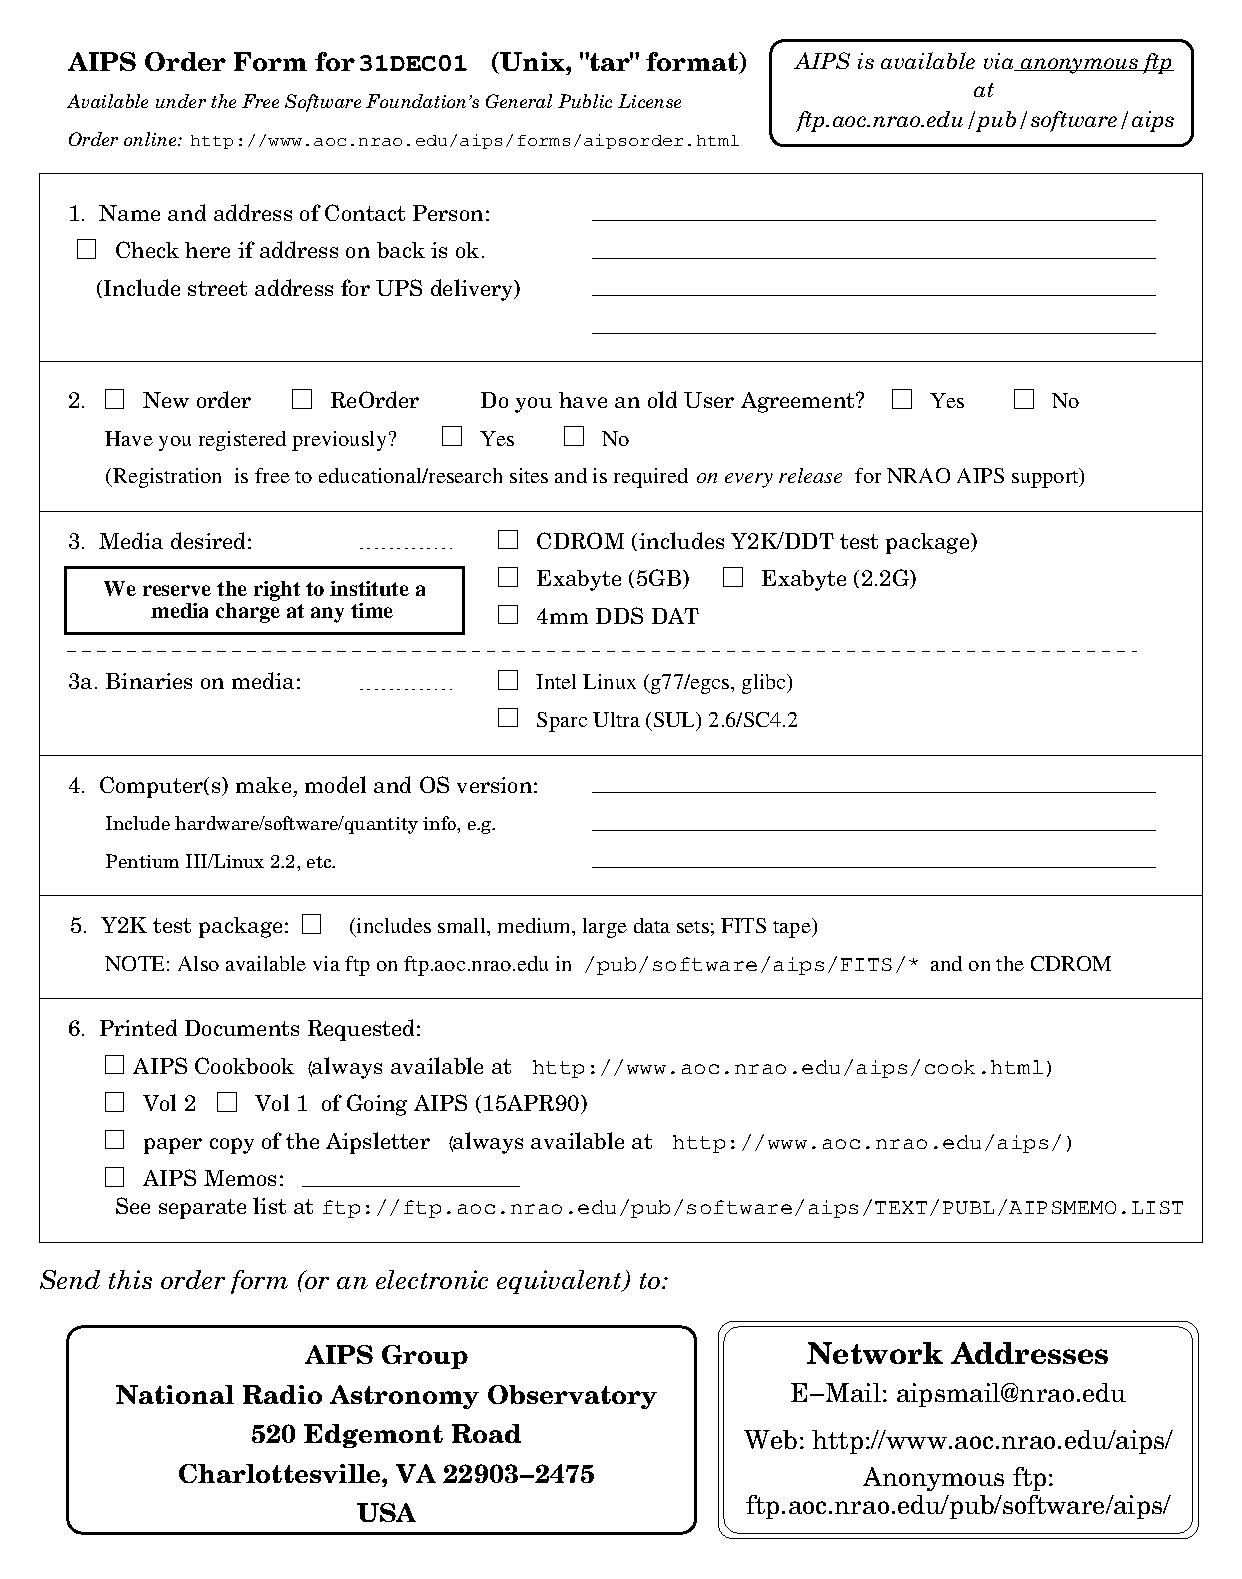
\includegraphics{FIG/AIPSORDER.PS}}}
\vfill\eject
  \vbox to 4.4in{
  \vfill
  \centerline{\resizebox{!}{2.6in}{\includegraphics{FIG/Mandrill.eps}}}
  \vspace{12pt}
  \centerline{{\huge \tt \AIPRELEASE}}
  \vspace{12pt}
  \vfill}
\phantom{...}
\centerline{\resizebox{!}{!}{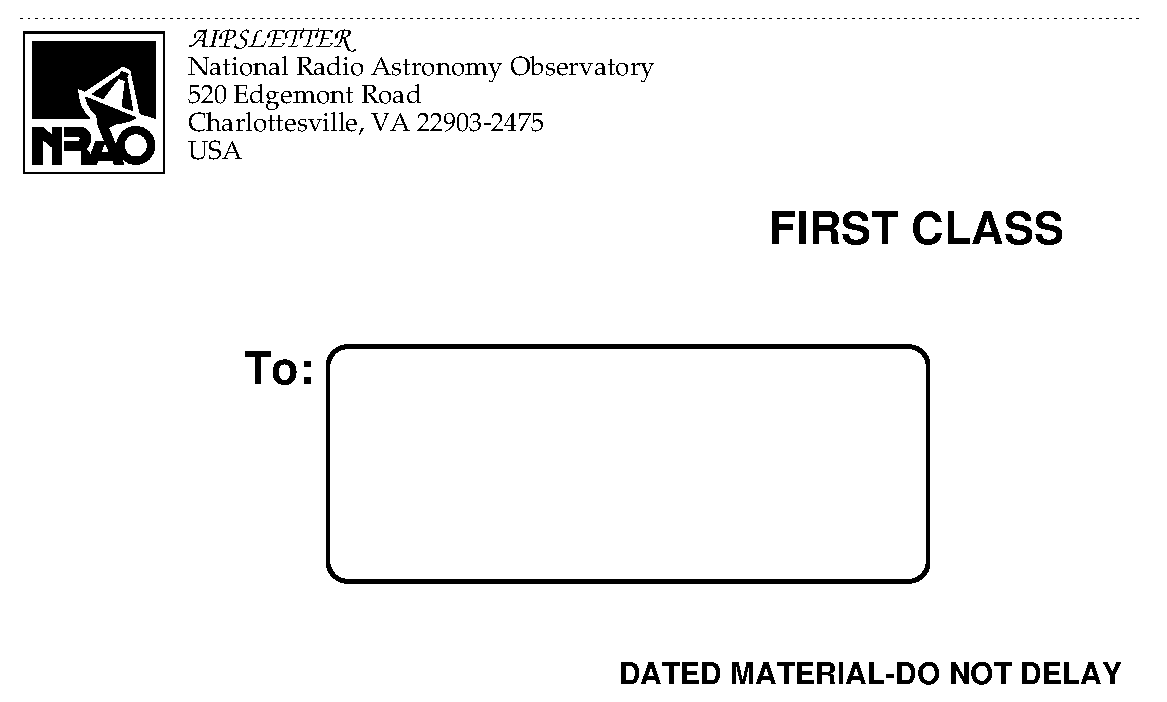
\includegraphics{FIG/AIPSLETM.PS}}}

\end{document}
